\documentclass[border=4pt]{standalone}
\usepackage{tikz}
\begin{document}

\noindent
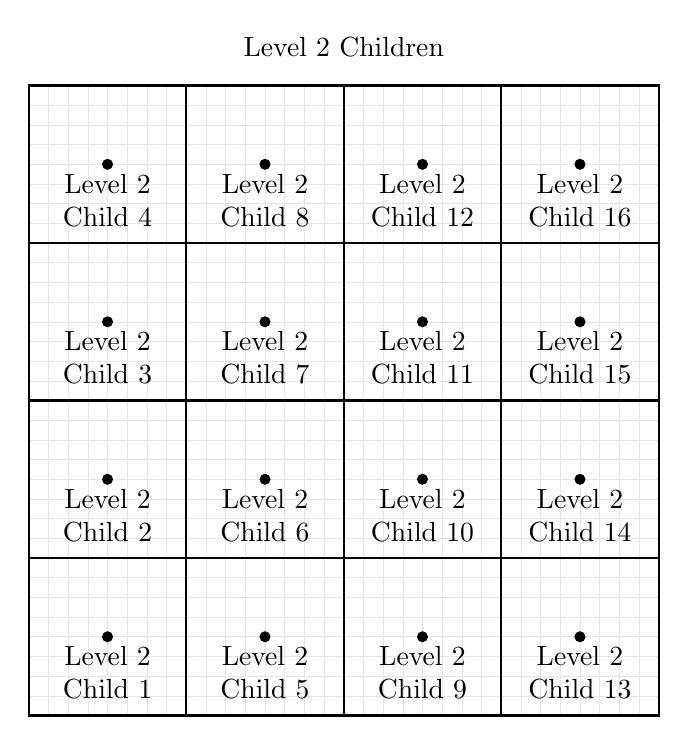
\begin{tikzpicture}[x=0.25cm,y=0.25cm]
  \draw[step=1,black!10,very thin] (0.0,0.0) grid (32.0,32.0);
  \node (TOPL) at (16,33) [above,align=center]  {Level 2 Children};

%% (let* ((p 5)
%%        (m (expt 2 p))
%%        (s 8)
%%        (n (1- (/ m s)))
%%        (i 0))
%%   (cl-loop for x from 0 upto n
%%            do (cl-loop for y from 0 upto n
%%                        do (cl-incf i)
%%                        do (let ((xc (+ (* s x) (/ s 2)))
%%                                 (yc (+ (* s y) (/ s 2)))
%%                                 (xr (+ (* s x)))
%%                                 (yr (+ (* s y))))
%%                             (insert (format "\\node (%02d%02d) at (%s,%s) [below,align=center]  {Level 2\\\\Child %d};\n"
%%                                          xc yc xc yc i))
%%                             (insert (format "\\fill (%d,%d) circle(2pt);\n"
%%                                             xc yc))
%%                             (insert (format "\\draw[thick] (%d,%d) rectangle (%d,%d);\n"
%%                                             xr yr (+ xr s) (+ yr s)))))))

  \node (0404) at (4,4) [below,align=center]  {Level 2\\Child 1};
  \fill (4,4) circle(2pt);
  \draw[thick] (0,0) rectangle (8,8);
  \node (0412) at (4,12) [below,align=center]  {Level 2\\Child 2};
  \fill (4,12) circle(2pt);
  \draw[thick] (0,8) rectangle (8,16);
  \node (0420) at (4,20) [below,align=center]  {Level 2\\Child 3};
  \fill (4,20) circle(2pt);
  \draw[thick] (0,16) rectangle (8,24);
  \node (0428) at (4,28) [below,align=center]  {Level 2\\Child 4};
  \fill (4,28) circle(2pt);
  \draw[thick] (0,24) rectangle (8,32);
  \node (1204) at (12,4) [below,align=center]  {Level 2\\Child 5};
  \fill (12,4) circle(2pt);
  \draw[thick] (8,0) rectangle (16,8);
  \node (1212) at (12,12) [below,align=center]  {Level 2\\Child 6};
  \fill (12,12) circle(2pt);
  \draw[thick] (8,8) rectangle (16,16);
  \node (1220) at (12,20) [below,align=center]  {Level 2\\Child 7};
  \fill (12,20) circle(2pt);
  \draw[thick] (8,16) rectangle (16,24);
  \node (1228) at (12,28) [below,align=center]  {Level 2\\Child 8};
  \fill (12,28) circle(2pt);
  \draw[thick] (8,24) rectangle (16,32);
  \node (2004) at (20,4) [below,align=center]  {Level 2\\Child 9};
  \fill (20,4) circle(2pt);
  \draw[thick] (16,0) rectangle (24,8);
  \node (2012) at (20,12) [below,align=center]  {Level 2\\Child 10};
  \fill (20,12) circle(2pt);
  \draw[thick] (16,8) rectangle (24,16);
  \node (2020) at (20,20) [below,align=center]  {Level 2\\Child 11};
  \fill (20,20) circle(2pt);
  \draw[thick] (16,16) rectangle (24,24);
  \node (2028) at (20,28) [below,align=center]  {Level 2\\Child 12};
  \fill (20,28) circle(2pt);
  \draw[thick] (16,24) rectangle (24,32);
  \node (2804) at (28,4) [below,align=center]  {Level 2\\Child 13};
  \fill (28,4) circle(2pt);
  \draw[thick] (24,0) rectangle (32,8);
  \node (2812) at (28,12) [below,align=center]  {Level 2\\Child 14};
  \fill (28,12) circle(2pt);
  \draw[thick] (24,8) rectangle (32,16);
  \node (2820) at (28,20) [below,align=center]  {Level 2\\Child 15};
  \fill (28,20) circle(2pt);
  \draw[thick] (24,16) rectangle (32,24);
  \node (2828) at (28,28) [below,align=center]  {Level 2\\Child 16};
  \fill (28,28) circle(2pt);
  \draw[thick] (24,24) rectangle (32,32);

\end{tikzpicture}

\end{document}




